	
%% bare_conf.tex
%% V1.3
%% 2007/01/11
%% by Michael Shell
%% See:
%% http://www.michaelshell.org/
%% for current contact information.
%%
%% This is a skeleton file demonstrating the use of IEEEtran.cls
%% (requires IEEEtran.cls version 1.7 or later) with an IEEE conference paper.
%%
%% Support sites:
%% http://www.michaelshell.org/tex/ieeetran/
%% http://www.ctan.org/tex-archive/macros/latex/contrib/IEEEtran/
%% and
%% http://www.ieee.org/

%%*************************************************************************
%% Legal Notice:
%% This code is offered as-is without any warranty either expressed or
%% implied; without even the implied warranty of MERCHANTABILITY or
%% FITNESS FOR A PARTICULAR PURPOSE! 
%% User assumes all risk.
%% In no event shall IEEE or any contributor to this code be liable for
%% any damages or losses, including, but not limited to, incidental,
%% consequential, or any other damages, resulting from the use or misuse
%% of any information contained here.
%%
%% All comments are the opinions of their respective authors and are not
%% necessarily endorsed by the IEEE.
%%
%% This work is distributed under the LaTeX Project Public License (LPPL)
%% ( http://www.latex-project.org/ ) version 1.3, and may be freely used,
%% distributed and modified. A copy of the LPPL, version 1.3, is included
%% in the base LaTeX documentation of all distributions of LaTeX released
%% 2003/12/01 or later.
%% Retain all contribution notices and credits.
%% ** Modified files should be clearly indicated as such, including  **
%% ** renaming them and changing author support contact information. **
%%
%% File list of work: IEEEtran.cls, IEEEtran_HOWTO.pdf, bare_adv.tex,
%%                    bare_conf.tex, bare_jrnl.tex, bare_jrnl_compsoc.tex
%%*************************************************************************

% *** Authors should verify (and, if needed, correct) their LaTeX system  ***
% *** with the testflow diagnostic prior to trusting their LaTeX platform ***
% *** with production work. IEEE's font choices can trigger bugs that do  ***
% *** not appear when using other class files.                            ***
% The testflow support page is at:
% http://www.michaelshell.org/tex/testflow/



% Note that the a4paper option is mainly intended so that authors in
% countries using A4 can easily print to A4 and see how their papers will
% look in print - the typesetting of the document will not typically be
% affected with changes in paper size (but the bottom and side margins will).
% Use the testflow package mentioned above to verify correct handling of
% both paper sizes by the user's LaTeX system.
%
% Also note that the "draftcls" or "draftclsnofoot", not "draft", option
% should be used if it is desired that the figures are to be displayed in
% draft mode.
%
\documentclass[10pt, conference, compsocconf]{IEEEtran}
% Add the compsocconf option for Computer Society conferences.
%
% If IEEEtran.cls has not been installed into the LaTeX system files,
% manually specify the path to it like:
% \documentclass[conference]{../sty/IEEEtran}





% Some very useful LaTeX packages include:
% (uncomment the ones you want to load)


% *** MISC UTILITY PACKAGES ***
%
%\usepackage{ifpdf}
% Heiko Oberdiek's ifpdf.sty is very useful if you need conditional
% compilation based on whether the output is pdf or dvi.
% usage:
% \ifpdf
%   % pdf code
% \else
%   % dvi code
% \fi
% The latest version of ifpdf.sty can be obtained from:
% http://www.ctan.org/tex-archive/macros/latex/contrib/oberdiek/
% Also, note that IEEEtran.cls V1.7 and later provides a builtin
% \ifCLASSINFOpdf conditional that works the same way.
% When switching from latex to pdflatex and vice-versa, the compiler may
% have to be run twice to clear warning/error messages.






% *** CITATION PACKAGES ***
%
%\usepackage{cite}
% cite.sty was written by Donald Arseneau
% V1.6 and later of IEEEtran pre-defines the format of the cite.sty package
% \cite{} output to follow that of IEEE. Loading the cite package will
% result in citation numbers being automatically sorted and properly
% "compressed/ranged". e.g., [1], [9], [2], [7], [5], [6] without using
% cite.sty will become [1], [2], [5]--[7], [9] using cite.sty. cite.sty's
% \cite will automatically add leading space, if needed. Use cite.sty's
% noadjust option (cite.sty V3.8 and later) if you want to turn this off.
% cite.sty is already installed on most LaTeX systems. Be sure and use
% version 4.0 (2003-05-27) and later if using hyperref.sty. cite.sty does
% not currently provide for hyperlinked citations.
% The latest version can be obtained at:
% http://www.ctan.org/tex-archive/macros/latex/contrib/cite/
% The documentation is contained in the cite.sty file itself.



\usepackage{arydshln}

%\usepackage{pdfpages}


% *** GRAPHICS RELATED PACKAGES ***
%
\ifCLASSINFOpdf
  \usepackage[pdftex]{graphicx}
  % declare the path(s) where your graphic files are
  \graphicspath{{../pdf/}{../jpeg/}}
  % and their extensions so you won't have to specify these with
  % every instance of \includegraphics
  \DeclareGraphicsExtensions{.pdf,.jpeg,.png}
\else
  % or other class option (dvipsone, dvipdf, if not using dvips). graphicx
  % will default to the driver specified in the system graphics.cfg if no
  % driver is specified.
  \usepackage[dvips]{graphicx}
  % declare the path(s) where your graphic files are
  \graphicspath{{../eps/}}
  % and their extensions so you won't have to specify these with
  % every instance of \includegraphics
  \DeclareGraphicsExtensions{.eps}
\fi
% graphicx was written by David Carlisle and Sebastian Rahtz. It is
% required if you want graphics, photos, etc. graphicx.sty is already
% installed on most LaTeX systems. The latest version and documentation can
% be obtained at: 
% http://www.ctan.org/tex-archive/macros/latex/required/graphics/
% Another good source of documentation is "Using Imported Graphics in
% LaTeX2e" by Keith Reckdahl which can be found as epslatex.ps or
% epslatex.pdf at: http://www.ctan.org/tex-archive/info/
%
% latex, and pdflatex in dvi mode, support graphics in encapsulated
% postscript (.eps) format. pdflatex in pdf mode supports graphics
% in .pdf, .jpeg, .png and .mps (metapost) formats. Users should ensure
% that all non-photo figures use a vector format (.eps, .pdf, .mps) and
% not a bitmapped formats (.jpeg, .png). IEEE frowns on bitmapped formats
% which can result in "jaggedy"/blurry rendering of lines and letters as
% well as large increases in file sizes.
%
% You can find documentation about the pdfTeX application at:
% http://www.tug.org/applications/pdftex





% *** MATH PACKAGES ***
%
\usepackage[cmex10]{amsmath}
% A popular package from the American Mathematical Society that provides
% many useful and powerful commands for dealing with mathematics. If using
% it, be sure to load this package with the cmex10 option to ensure that
% only type 1 fonts will utilized at all point sizes. Without this option,
% it is possible that some math symbols, particularly those within
% footnotes, will be rendered in bitmap form which will result in a
% document that can not be IEEE Xplore compliant!
%
% Also, note that the amsmath package sets \interdisplaylinepenalty to 10000
% thus preventing page breaks from occurring within multiline equations. Use:
%\interdisplaylinepenalty=2500
% after loading amsmath to restore such page breaks as IEEEtran.cls normally
% does. amsmath.sty is already installed on most LaTeX systems. The latest
% version and documentation can be obtained at:
% http://www.ctan.org/tex-archive/macros/latex/required/amslatex/math/
\usepackage{romannum}


\usepackage{algorithm}
\usepackage[algo2e]{algorithm2e}
% *** SPECIALIZED LIST PACKAGES ***
%
%\usepackage{algorithmic}
% algorithmic.sty was written by Peter Williams and Rogerio Brito.
% This package provides an algorithmic environment fo describing algorithms.
% You can use the algorithmic environment in-text or within a figure
% environment to provide for a floating algorithm. Do NOT use the algorithm
% floating environment provided by algorithm.sty (by the same authors) or
% algorithm2e.sty (by Christophe Fiorio) as IEEE does not use dedicated
% algorithm float types and packages that provide these will not provide
% correct IEEE style captions. The latest version and documentation of
% algorithmic.sty can be obtained at:
% http://www.ctan.org/tex-archive/macros/latex/contrib/algorithms/
% There is also a support site at:
% http://algorithms.berlios.de/index.html
% Also of interest may be the (relatively newer and more customizable)
% algorithmicx.sty package by Szasz Janos:
% http://www.ctan.org/tex-archive/macros/latex/contrib/algorithmicx/




% *** ALIGNMENT PACKAGES ***
%
%\usepackage{array}
% Frank Mittelbach's and David Carlisle's array.sty patches and improves
% the standard LaTeX2e array and tabular environments to provide better
% appearance and additional user controls. As the default LaTeX2e table
% generation code is lacking to the point of almost being broken with
% respect to the quality of the end results, all users are strongly
% advised to use an enhanced (at the very least that provided by array.sty)
% set of table tools. array.sty is already installed on most systems. The
% latest version and documentation can be obtained at:
% http://www.ctan.org/tex-archive/macros/latex/required/tools/


%\usepackage{mdwmath}
%\usepackage{mdwtab}
% Also highly recommended is Mark Wooding's extremely powerful MDW tools,
% especially mdwmath.sty and mdwtab.sty which are used to format equations
% and tables, respectively. The MDWtools set is already installed on most
% LaTeX systems. The lastest version and documentation is available at:
% http://www.ctan.org/tex-archive/macros/latex/contrib/mdwtools/


% IEEEtran contains the IEEEeqnarray family of commands that can be used to
% generate multiline equations as well as matrices, tables, etc., of high
% quality.


%\usepackage{eqparbox}
% Also of notable interest is Scott Pakin's eqparbox package for creating
% (automatically sized) equal width boxes - aka "natural width parboxes".
% Available at:
% http://www.ctan.org/tex-archive/macros/latex/contrib/eqparbox/





% *** SUBFIGURE PACKAGES ***
%\usepackage[tight,footnotesize]{subfigure}
% subfigure.sty was written by Steven Douglas Cochran. This package makes it
% easy to put subfigures in your figures. e.g., "Figure 1a and 1b". For IEEE
% work, it is a good idea to load it with the tight package option to reduce
% the amount of white space around the subfigures. subfigure.sty is already
% installed on most LaTeX systems. The latest version and documentation can
% be obtained at:
% http://www.ctan.org/tex-archive/obsolete/macros/latex/contrib/subfigure/
% subfigure.sty has been superceeded by subfig.sty.



%\usepackage[caption=false]{caption}
\usepackage[caption=false,font=footnotesize]{subfig}
% subfig.sty, also written by Steven Douglas Cochran, is the modern
% replacement for subfigure.sty. However, subfig.sty requires and
% automatically loads Axel Sommerfeldt's caption.sty which will override
% IEEEtran.cls handling of captions and this will result in nonIEEE style
% figure/table captions. To prevent this problem, be sure and preload
% caption.sty with its "caption=false" package option. This is will preserve
% IEEEtran.cls handing of captions. Version 1.3 (2005/06/28) and later 
% (recommended due to many improvements over 1.2) of subfig.sty supports
% the caption=false option directly:
%\usepackage[caption=false,font=footnotesize]{subfig}
%
% The latest version and documentation can be obtained at:
% http://www.ctan.org/tex-archive/macros/latex/contrib/subfig/
% The latest version and documentation of caption.sty can be obtained at:
% http://www.ctan.org/tex-archive/macros/latex/contrib/caption/




% *** FLOAT PACKAGES ***
%
%\usepackage{fixltx2e}
% fixltx2e, the successor to the earlier fix2col.sty, was written by
% Frank Mittelbach and David Carlisle. This package corrects a few problems
% in the LaTeX2e kernel, the most notable of which is that in current
% LaTeX2e releases, the ordering of single and double column floats is not
% guaranteed to be preserved. Thus, an unpatched LaTeX2e can allow a
% single column figure to be placed prior to an earlier double column
% figure. The latest version and documentation can be found at:
% http://www.ctan.org/tex-archive/macros/latex/base/



%\usepackage{stfloats}
% stfloats.sty was written by Sigitas Tolusis. This package gives LaTeX2e
% the ability to do double column floats at the bottom of the page as well
% as the top. (e.g., "\begin{figure*}[!b]" is not normally possible in
% LaTeX2e). It also provides a command:
%\fnbelowfloat
% to enable the placement of footnotes below bottom floats (the standard
% LaTeX2e kernel puts them above bottom floats). This is an invasive package
% which rewrites many portions of the LaTeX2e float routines. It may not work
% with other packages that modify the LaTeX2e float routines. The latest
% version and documentation can be obtained at:
% http://www.ctan.org/tex-archive/macros/latex/contrib/sttools/
% Documentation is contained in the stfloats.sty comments as well as in the
% presfull.pdf file. Do not use the stfloats baselinefloat ability as IEEE
% does not allow \baselineskip to stretch. Authors submitting work to the
% IEEE should note that IEEE rarely uses double column equations and
% that authors should try to avoid such use. Do not be tempted to use the
% cuted.sty or midfloat.sty packages (also by Sigitas Tolusis) as IEEE does
% not format its papers in such ways.





% *** PDF, URL AND HYPERLINK PACKAGES ***
%
%\usepackage{url}
% url.sty was written by Donald Arseneau. It provides better support for
% handling and breaking URLs. url.sty is already installed on most LaTeX
% systems. The latest version can be obtained at:
% http://www.ctan.org/tex-archive/macros/latex/contrib/misc/
% Read the url.sty source comments for usage information. Basically,
% \url{my_url_here}.





% *** Do not adjust lengths that control margins, column widths, etc. ***
% *** Do not use packages that alter fonts (such as pslatex).         ***
% There should be no need to do such things with IEEEtran.cls V1.6 and later.
% (Unless specifically asked to do so by the journal or conference you plan
% to submit to, of course. )


% correct bad hyphenation here
\hyphenation{op-tical net-works semi-conduc-tor}
\usepackage{subfloat}
%\usepackage[labelfont=bf]{caption}
%\usepackage{subcaption}
\usepackage{amsmath}
\usepackage{amssymb}
\usepackage{multirow}
\usepackage[flushleft]{threeparttable}

\begin{document}

\title{Clustering Metagenome Sequences Using Canopies}

\author{\IEEEauthorblockN{Mohammad Arifur Rahman, Nathan LaPierre, Huzefa Rangwala and Daniel Barbara}
\IEEEauthorblockA{
Department of Computer Science\\
George Mason University\\
Fairfax, VA, United States\\
Email: mrahma23@gmu.edu, nlapier2@gmu.edu, rangwala@cs.gmu.edu and dbarbara@gmu.edu}
}
% make the title area
\maketitle

\begin{abstract}
	
Advances in genome technologies 
has allowed for the 
collective sequencing of co-existing 
microbial communities (Metagenomics) that are ubiquitous 
across environments like the soil, ocean and human body.
%
Metagenomics has 
spurred the development of several 
bioinformatics approaches for analyzing 
the diversity, abundance, function and role of the 
different organisms 
within these communities. 
%
%As an example,  metagenomics allows for the analysis of the pathogenic role played by the microbial organisms within the human host and has implications for betterment of health and drug discovery. 


We present 
a fast and scalable 
clustering algorithm
for analyzing 
large-scale metagenome sequence
data. Our approach 
achieves efficiency 
by  
partitioning the large number of sequence reads into 
groups (called canopies) using locality sensitive 
hashing.  This 
initial approximate assignment of sequence reads to 
canopies is then 
refined by using 
state-of-the-art
sequence clustering 
algorithms. This
two-phase 
approach allows for the
use  of 
our developed algorithms as a pre-processing phase for 
computationally expensive 
clustering 
algorithms. Using the clusters as surrogates for 
Operational Taxonomic Units (OTUs) we 
estimate  the biodiversity within 
a community sample.
%
The Canopy-based clustering 
algorithm is evaluated on synthetic and real 
world 16S and whole 
metagenome  benchmarks. We demonstrate the ability 
of our proposed approach to  
determine meaningful OTU assignments and observe
significant speedup with regards 
to run time when combined with three 
different clustering algorithms. 


\end{abstract}

\begin{IEEEkeywords}
Clustering, Canopy, Metagenome, 16S, Biodiversity 
\end{IEEEkeywords}

% For peer review papers, you can put extra information on the cover
% page as needed:
% \ifCLASSOPTIONpeerreview
% \begin{center} \bfseries EDICS Category: 3-BBND \end{center}
% \fi
%
% For peerreview papers, this IEEEtran command inserts a page break and
% creates the second title. It will be ignored for other modes.
\IEEEpeerreviewmaketitle

\section{Introduction}
\label{intro}

% Microorganism and it's Importance + what is metagenome
% HR Editing [Nice work Mohammad]

A large portion of the  earth's biomass 
comprises trillions of tiny  microorganisms 
with varying  biodiversity.  Communities
of interacting microbes  exists in several 
ecosystems varying from the soil, ocean 
and human body \cite{MARHumanMicro}; and though, most of 
them are beneficial to the host some are known to cause 
unwanted conditions and can be linked to cause of 
diseases in the host \cite{MARTurnbaugh}. 
%
\emph{Metagenomics} is the 
sequencing of the collective DNA  of 
microbial organisms coexisting as communities. Analyzing 
metagenomes has provided an unprecedented 
opportunity to understand the diversity, role and 
function of these organisms within different 
clinical and ecological environments \cite{MARHumanGut}\cite{MARMihaiPop}.


However, sequencing technologies do not deliver the 
complete genome of an organism (millions in length), but 
large number of short contiguous 
subsequences called \emph{reads} of length $75$ to $500$ in 
random order. Sequencing communities of genomes 
leads to additional challenges because reads 
from different microbes are mixed together; and 
upfront  the composition of a community in terms of 
abundance and identity of microbial species
is unknown \cite{MARMetaChallenge}. Sequencing technologies also 
produce large 
datasets that range from Gigabytes (GB) to Terabytes (TB).  Alternatively, 
targeted metagenome sequencing  that 
involves sequencing of \emph{marker genes} has been 
popular for the characterization of these communities. 16S and 18S 
sequences are repetitive marker genes within microbial genomes that 
are generally conserved but 
have slight 
variations in their sequences 
that allow them to be separated into different 
taxonomic groups \cite{MAR16S}. 


In the past few years, several unsupervised 
clustering algorithms have been developed and
used for the analysis of large-scale targeted and whole 
metagenome sequence reads 
(reviewed in Section \ref{sec:Literature}). The 
unsupervised grouping  of similar sequences from the 
16S/18S genes is referred as \emph{binning} and 
allows for the estimation of biodiversity within a sample. Binning 
leads to assignment of similar sequences within groups called \emph{Operational Taxonomic Units (OTUs)} \cite{MAROTU}. Microbial OTUs are generally 
ecologically consistent across the hosts regardless of the 
clustering approaches \cite{MAROTUConsistant}. 

% What have we done and how it is better

In this paper we develop an 
efficient clustering algorithm based on Canopy Clustering \cite{MARCanopy} which can be used as a pre-clustering  
step with any state-of-the-art sequence clustering algorithm. Specifically, 
our approach identifies canopies with a greedy procedure and a 
fast sequence distance metric based on locality 
sensitive hashing \cite{MARLshRef2}. Sequences within the canopies are 
considered as an initial partition (or grouping) of data which can be 
further refined by applying expensive and accurate clustering 
algorithms. Our developed approach treats each canopies independently 
allowing for easy parallelization.

We present experimental results on 
real and synthetic metagenome sequence
benchmarks. We show that the 
use of Canopy Clustering (CC) in combination 
with UCLUST \cite{MARuclust}, SUMACLUST \cite{MARSumaclust} and 
SWARM \cite{MARSwarm2} leads to improved run 
time efficiency by 12.19, 21.09 and 18.61 times with accurate clustering results, respectively. We also demonstrate that our 
developed approach is scalable for large datasets with 
increased number of processors. The 
source code is freely available on Github\footnote{https://github.com/mrahma23/LSH-Canopy} for public use. 

          

\section{Literature Review}
\label{sec:Literature}

In the past decade, several 
sequence clustering methods have been developed and
used widely for metagenome sequences. A comprehensive survey 
by Kopylova et. al. \cite{MARopenDeNovo} benchmarks 
various  approaches 
including UCLUST \cite{MARuclust}, SWARM \cite{MARSwarm2}, 
SUMACLUST \cite{MARSumaclust} and MOTHUR \cite{MARMothur}. 

CD-HIT \cite{MARCDhit} is a 
general purpose sequence clustering algorithm that 
follows an incremental, greedy approach. CD-HIT uses 
pairwise sequence alignment to find similar 
sequences. UCLUST \cite{MARuclust} is similar to CD-HIT but 
achieves a significant speedup over CD-HIT by using seeds (fixed length gapless subsequences) for 
performing pairwise sequence comparisons. MC-LSH \cite{MARMetaLSH} utilizes 
an efficient locality sensitive based hashing function to 
approximate the pairwise sequence similarity. MC-MinH \cite{MARMcMinH} uses 
min-wise \cite{MARMinWise} hashing along with 
greedy clustering to group 16S and whole metagenome sequences. Mash \cite{MAROtherMinH}, uses MinHash 
locality sensitive hashing 
to reduce large sequences to a representative sketch and 
estimate
pairwise distances. Other methods for clustering sequence 
reads include TOSS \cite{MARToss}, AbundanceBin \cite{MARAbundant} and CompostBin \cite{MARCompost}. All unique 
kmers are first grouped in TOSS and then clusters are merged 
based on kmer repetitions. In AbundanceBin, reads are modeled as a 
mixture of Poisson distributions. Expectation Maximization (EM) algorithm 
is used to infer model parameters for the final clustering. Principal 
component analysis is used within CompostBin to project the data into a 
lower dimensional space
followed with a graph partitioning approach. MOTHUR \cite{MARMothur} uses a pairwise distance matrix as 
input and performs hierarchical clustering. 

%
SWARM \cite{MARSwarm2} uses exhaustive single-linkage clustering 
based on optimal sequence alignment. Sequences that are less than 
a certain distance from any other other sequence in the cluster are 
clustered together. SWARM attempts to reduce the impact of clustering 
parameters on the resulting OTUs by avoiding arbitrary 
thresholds and input sequence ordering dependencies. SWARM builds 
an initial set of OTUs  by 
iteratively agglomerating similar amplicons. The amplicon abundance values are used to reveal 
OTUs’ internal structures and 
break them into sub-OTUs.
%
SUMACLUST \cite{MARSumaclust} is similar to UCLUST and uses 
a  greedy strategy to 
incrementally construct clusters by comparing an 
abundance-ordered list of input sequences against the 
representative set of already-chosen sequences.  UCLUST, SWARM and SUMACLUST are 
considered to be 
state-of-the-art metagenome sequence clustering methods by a 
benchmarking study \cite{MARopenDeNovo}.  As such, we compare the performance of our developed method with these three approaches. 


%In this study we developed h  using Canopies \cite{MARCanopy}. The 
%developed approach can be used as a pre-processing step for
%other state-of-art sequence clustering
%algorithms to improve efficiency and also retains correctness in clustering.

\section{Methods}
\label{sec:Methods}
\subsection{\textbf{Overview}}

% Question - is this repetive ? 
% HR

Figure \ref{fig:flowchart} shows an overview of our 
proposed canopy clustering algorithm.  Sequence reads are represented with \textit{kmers} defined as contiguous subsequence of 
length $k$. One of the input reads is chosen randomly 
as the canopy centroid. Then we compute the distances of other reads to 
this canopy centroid. Two thresholds are used in Canopy clustering algorithm. If the 
distance is less than a \emph{tight} threshold ($T2$) we assign the read to the canopy and that
read will not be considered for another canopy. Otherwise, if a distance is less than a \emph{soft} threshold ($T1$) we assign the 
read to the canopy but that read will be available for another 
canopy. This process continues until all sequence reads are
assigned to atleast one canopy. For fast canopy assignment we use a random projection based 
technique. Specifically, we use Locality Sensitive Hash (LSH) to compute pairwise distances. More accurate clustering methods are 
used to sub-cluster each canopy in parallel. The sub-clustering method considers only the members within 
the canopy which significantly 
reduces pairwise distance computations.

\begin{figure}
	\centering
	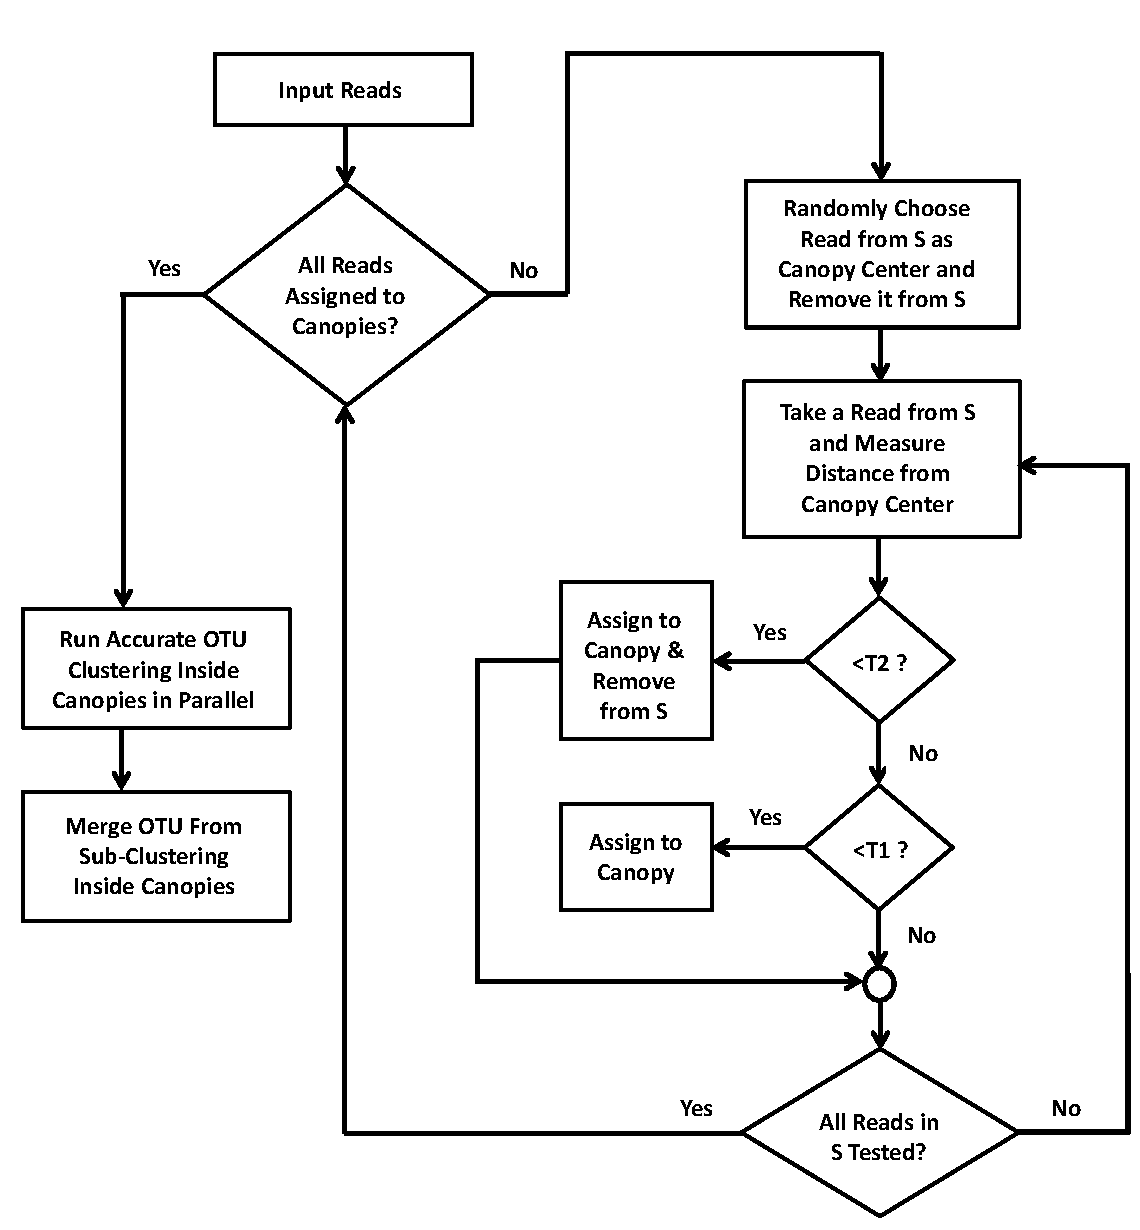
\includegraphics[width=\linewidth,height=10cm]{flowchart.pdf}	
	\caption{Workflow of Canopy Clustering for Large Scale Metagenome Data}
	\label{fig:flowchart}
\end{figure}

\subsection{\textbf{Canopy Clustering}}

Canopy Clustering \cite{MARCanopy} is an efficient approximate 
clustering algorithm often used as pre-processing step for other accurate and expensive clustering methods like  K-means or Hierarchical clustering. It
is intended to speed up the 
clustering operations for 
large data sets, where standard clustering algorithms may be 
impractical due to  run time and memory requirements. 
%
For a dataset with $N$ instances, the 
worst case calculations without canopy 
clustering is $O(N^2)$. Using canopy clustering, 
assuming the number of 
canopies is set to 
$k$; the 
worst case calculations with canopy clustering is $\sum_{i=1}^{k}(c_i)^2$ where $c_i$ is the number of instances within $i$-th canopy.


Canopy clustering uses two distance 
thresholds, (\romannum{1}) \textit{soft} threshold $T1$ and (\romannum{2}) \textit{tight} threshold $T2$. If data point $p_1$ is within the 
soft distance threshold $T1$ with centroid $p_2$ then $p_1$ will reside in same canopy as $p_2$ but $p_1$ may belong to other 
canopies assuming that it has only met soft threshold and best match is yet to be found. Thus one data point may belong to multiple canopies. However, 
if data point $p_1$ is within the tight distance threshold $T2$ with centroid $p_2$ then canopy clustering assigns $p_1$ to the same canopy as $p_2$ and stops 
  assigning $p_1$ to any other canopy assuming that tight threshold has been met and 
  best canopy assignment for $p_1$ has been found. Canopy centroids are selected randomly until all data points are
  assigned to at least one canopy. 


\subsection{\textbf{Locality Sensitive Hashing}}

Canopies are intended to reduce pairwise distance calculations. As such, canopy clustering 
should be efficient which requires a fast and approximate distance measure. Locality Sensitive Hashing (LSH) \cite{MARLshRef2} provides a solution 
for the approximate or exact near neighbors search problem. Given,  a space S of points with a 
  distance measure $d(x,y)$; a family $H$ of hash functions is said to be $(d1, d2, p1, p2)$-sensitive for any x and 
  y in S: if $d(x, y)<d1$, then the probability over all $h\in{H}$, that $h(x)=h(y)$ is at least $p1$ and if $d(x, y)>d2$ , then the probability over 
  all $h\in{H}$, that $h(x)=h(y)$ is at most $p2$. LSH provides a fast approximate distance measure while reducing 
  data dimensionality making it 
  appropriate for Canopy clustering for 
  16S and whole metagenomic data.

We construct the LSH family with bit sampling \cite{indyk1998approximate}. The normalized kmers frequency based feature vectors of sequence reads 
were first projected into $d$ dimensional vectors in $\{0,1\}^d$ space. Given an 
input vector $v$ and a random hyperplane defined by $r$, we let $h(v)=\{0,1\}$ based on $sgn(v\cdot{r})=\pm{1}$ that indicates on which 
side of the hyperplane $v$ lies. Each possible choice of $r$ defines a single function. Let $H$ be the set of all 
such functions. For any $h_i\in{H}$ and for any two data $x,y$ the probability that $x$ and $y$ \emph{agree} on $i^{th}$ positions of their 
respective $d$-length binary vector is

\begin{equation}
P[h_i(x)=h_i(y)]=1-\frac{distance(h_i(x),h_i(y))}{d} 
\end{equation}

where \emph{distance} is the hamming distance and $d$ is the number of bits. Hence $H=\{h_1,h_2,...,h_d\}$ is a $(d_1,d_2,1-d_1/d,1-d2/d)$ sensitive LSH family. The 
random projection and hamming distance calculation is computationally cheap and efficient making it 
suitable for fast partitioning of large volume of 
sequence reads. 

%that more expensive clustering can be done in parallel.

%%Moreover, this projection and distance scheme is computationally inexpensive than another popular alternative for LSH known as MinHash \cite{broder1997resemblance}. MinHash provides $n!$ choices for hash functions in LSH family where $n$ is the total number of kgrams. Whereas our scheme generates only $d<<n!$ hash functions where $d$ can be easily estimated by sampling and validation based on 16S and metagenomic data.  

\subsection{\textbf{Sub-Clustering Inside Canopies}}
\label{sub-cluster}

Canopy clustering  makes initial approximate partitions of the dataset and reduces pairwise
distance computations. Each of these partitions can be further clustered in parallel and independendtly 
with  expensive (but accurate)  clustering methods. 
%
We use UCLUST \cite{MARuclust}, SUMACLUST \cite{MARSumaclust} or 
SWARM \cite{MARSwarm2}  as accurate and 
expensive sub-clustering methods  for the different 
canopies in this study. 


\subsection{\textbf{Merging results from Canopies}}

Each cluster (OTU) is represented by the Longest Common Subsequence of all member sequences. The final step of 
our proposed framework is to merge the 
OTU representations generated by the 
canopies. According to Canopy cluster algorithm a single data point may belong to multiple canopies as long as the soft threshold is met. As a result similar OTU representations may appear from multiple canopies. To eliminate redundancy we run UCLUST on the OTU representations.

In this paper,  the Canopy clustering (CC)  approach 
integrated with UCLUST, SUMACLUST and SWARM 
are represented as CC$_{UCLUST}$, CC$_{SUMACLUST}$ and CC$_{SWARM}$, respectively. % where the term CC stands for Canopy Clustering. 

\section{Experimental Evaluation}
\label{sec:Experimental}

\subsection{\textbf{Dataset Description}}

To evaluate the performance of our proposed approach we use previously 
published synthetic and real world 16S, 18S and metagenome sequence benchmarks. Key statistics and relevant 
information regarding these datasets are presented in Table \ref{table:finaltabledataset}. 

\begin{table}[htb] 
	%\centering 
	\caption{\textbf{Dataset Statistics}}
	\label{table:finaltabledataset}
	\resizebox{\columnwidth}{!}{%
	\begin{tabular}{|l| c c c c|} 
		\hline
		\multirow{2}{*}{{\bf{Datasets}}} & \multirow{2}{*}{{\bf{Type}}} & {\bf{\# of}} & {\bf{\# of}}  & \multirow{2}{*}{\bf{Platform}}\\
		 & & \bf{Reads} & \bf{Samples} & \\
		\hline
		{Bokulich$_2$} \cite{MARmockDatasetRef} & M & 6,938,836 & 4 & H\\
		{Bokulich$_3$} \cite{MARmockDatasetRef} & M & 3,594,237 & 4 & H\\
		{Bokulich$_6$} \cite{MARmockDatasetRef} & M & 250,903 & 1 & H\\
		{Canadian Soil} \cite{MARcanadianSoil} & R & 2,966,053 & 13 & H\\
		{Body Sites} \cite{MARbodySites} & R & 886,630 & 602 & G\\
		{Global Soil} \cite{MARglobalSoil} & R & 9,252,764 & 57 & H\\
		{Liver Cirrhosis} \cite{qin2014alterations} & R & 6,117,828,130 & 232 & H\\ 
		\hline
	\end{tabular}
	}
	\begin{tablenotes}
		\item Table shows information about dataset used in this study. M, R, H and G represent Mock, Real World, HiSeq and GS-FLX, respectively.		
	\end{tablenotes}
\end{table}	


\begin{table*}[t]
	\centering 
	\caption{\textbf{Performance Comparison [$F$-Score and Pearson Correlation Coefficient ($\rho$)]}} 
	\label{table:performanceTable}
	
	\scalebox{0.82}{
		
		\begin{tabular}{|l|c c c c| c c c c c|}
			
			\hline
			
			\textbf{Methods} & \textbf{Comparison Metric} & \multicolumn{8}{c|}{\textbf{Datasets}}\\
			
			\cline{3-10}
			
			& & \multicolumn{3}{c|}{\textit{Synthetic}} & \multicolumn{5}{c|}{\textit{Real World}}\\ 
			
			\cline{3-10}
			
			%&  & Bokulich$_2$ & Bokulich$_3$ & Bokulich$_6$ & Body Sites & Canadian Soil & Global Soil\\
			
			&  &  &  & & & & & Liver Cirrhosis & Liver Cirrhosis\\
			
			& & Bokulich$_2$ & Bokulich$_3$ & Bokulich$_6$ & Body Sites & Canadian Soil & Global Soil & Metagenome & Metagenome\\
			
			& & & & & & & & (Sampled 3M) & (Sampled 30M)\\
			
			\hline
			
			\multirow{1}{*}{UCLUST} & $F$-Measure & 0.39 & 0.40 & 0.51 & $N/A$ & $N/A$ & $N/A$ & $N/A$ & $N/A$\\
			
			\hdashline
			
			\multirow{2}{*}{CC$_{UCLUST}$} & $F$-Measure & \textit{\textbf{0.39}} & \textit{\textbf{0.41}} & \textit{\textbf{0.52}} & $N/A$ & $N/A$ & $N/A$ & $N/A$ & $N/A$\\
			& ($\rho$) with Respect to UCLUST & \textit{\textbf{0.9831}} & \textit{\textbf{0.9753}} & \textit{\textbf{0.9831}} & \textit{\textbf{0.9682}} & \textit{\textbf{0.8419}} & \textit{\textbf{0.9824}} & \textit{\textbf{0.9216}} & \textit{\textbf{0.9072}}\\
			
			\hline 
			
			\multirow{1}{*}{SUMACLUST} & $F$-Measure & 0.40 & 0.41 & 0.51 & $N/A$ & $N/A$ & $N/A$ & $N/A$ & $N/A$\\
			
			\hdashline
			
			\multirow{2}{*}{CC$_{SUMACLUST}$} & $F$-Measure & \textit{\textbf{0.41}} & \textit{\textbf{0.42}} & \textit{\textbf{0.51}} & $N/A$ & $N/A$ & $N/A$ & $N/A$ & $N/A$\\
			& ($\rho$) with Respect to SUMACLUST & \textit{\textbf{0.9709}} & \textit{\textbf{0.9813}} & \textit{\textbf{0.9538}} & \textit{\textbf{0.9518}} & \textit{\textbf{0.7643}} & \textit{\textbf{0.8714}} & \textit{\textbf{0.9281}} & \textit{\textbf{0.8614}}\\ 
			
			\hline
			
			\multirow{1}{*}{SWARM} & $F$-Measure & 0.46 & 0.48 & 0.55 & $N/A$ & $N/A$ & $N/A$ & $N/A$ & $N/A$\\
			
			\hdashline
			
			\multirow{2}{*}{CC$_{SWARM}$} & $F$-Measure & \textit{\textbf{0.46}} & \textit{\textbf{0.49}} & \textit{\textbf{0.56}} & $N/A$ & $N/A$ & $N/A$ & $N/A$ & $N/A$\\
			& ($\rho$) with Respect to SWARM & \textit{\textbf{0.9817}} & \textit{\textbf{0.97861}} & \textit{\textbf{0.9251}} & \textit{\textbf{0.9648}} & \textit{\textbf{0.7581}} & \textit{\textbf{0.9143}} & \textit{\textbf{0.9263}} & \textit{\textbf{0.8533}}\\
			
			\hline
			
		\end{tabular}
	}
	\small
	\begin{tablenotes}
		\item Table shows values of $F$-measures and Pearson Correlation Coefficient ($\rho$-value) of UCLUST, SUMACLUST, SWARM and their respective versions with Canopy clustering. $F$-measures is only available for synthetic datasets but not for real world datasets since no ground truths like known taxonomic profiles are available for them. $\rho$-value was calculated based on the taxonomy profiles at Genus level generated from clustered OTUs provided by a method and it's corresponding Canopy counterpart. Higher $F$-measures reflect better clustering by adhering to ground truth. Higher $\rho$-values reflect stronger correlation between taxonomic profiles. Higher F-scores and $\rho$ values are represented with bold and italic letters.         
	\end{tablenotes}
	
\end{table*}


\begin{table*}[t]
	\centering 
	\caption{\textbf{Biodiversity Comparison [Faith’s phylogenetic diversity metric (PD), Shannon and Simpson]}} 
	\label{table:bioDiversityTable}
	
	\scalebox{0.80}{
		
		\begin{tabular}{|c|c c c c| c c c c|}
			
			\hline
			
			\textbf{Methods} & \textbf{Comparison Metric} & \multicolumn{7}{c|}{\textbf{Datasets}}\\
			
			\cline{3-9}
			
			& & \multicolumn{3}{c|}{\textit{Synthetic}} & \multicolumn{4}{c|}{\textit{Real World}}\\ 
			
			\cline{3-9}
			
			&  &  &  & & & & & Liver Cirrhosis\\
			
			& & Bokulich$_2$ & Bokulich$_3$ & Bokulich$_6$ & Body Sites & Canadian Soil & Global Soil & Metagenome\\
			
			& & & & & & & & (Sampled 3M)\\
			
			\hline
			
			\multirow{3}{*}{UCLUST} & PD Range & $\left[171.95-221.85\right]$ & $\left[186.90-212.84\right]$ & $\left[104.51-104.51\right]$ & $\left[1.46-46.79\right]$ & $\left[0.30-1352.73\right]$ & $\left[2.98-3.29\right]$ & $\left[3.14-51.47\right]$\\ 
			& Shannon Range & $\left[2.52-3.51\right]$ & $\left[2.43-3.54\right]$ & $\left[5.87-5.87\right]$ & $\left[0.29-7.67\right]$ & $\left[2.32-7.86\right]$ & $\left[1.84-8.30\right]$ & $\left[0.27-5.77\right]$\\
			& Simpson Range & $\left[0.55-0.75\right]$ & $\left[0.55-0.76\right]$ & $\left[0.96-0.96\right]$ & $\left[0.049-0.98\right]$ & $\left[0.80-0.99\right]$ & $\left[0.0-0.98\right]$ & $\left[0.02-0.97\right]$\\
			
			& & & & & & & & \\
			
			\multirow{3}{*}{CC$_{UCLUST}$} & PD Range & $\left[164.79-217.72\right]$ & $\left[169.41-198.36\right]$ & $\left[109.33-109.33\right]$ & $\left[2.37-47.13\right]$ & $\left[0.52-1419.31\right]$ & $\left[3.02-3.81\right]$ & $\left[4.61-53.29\right]$\\
			& Shannon Range & $\left[2.61-3.83\right]$ & $\left[2.92-3.91\right]$ & $\left[6.41-6.41\right]$ & $\left[0.93-7.13\right]$ & $\left[3.26-7.61\right]$ & $\left[3.72-7.38\right]$ & $\left[0.13-6.17\right]$\\
			& Simpson Range & $\left[0.64-0.87\right]$ & $\left[0.56-0.93\right]$ & $\left[0.96-0.96\right]$ & $\left[0.081-0.99\right]$ & $\left[0.84-0.99\right]$ & $\left[0.21-0.99\right]$ & $\left[0.09-0.98\right]$\\
			
			\hline
			
			\multirow{3}{*}{SUMACLUST} & PD Range & $\left[106.00-162.78\right]$ & $\left[142.85-174.19\right]$ & $\left[89.22-89.22\right]$ & $\left[0.93-39.47\right]$ & $\left[0.59-1279.29\right]$ & $\left[2.98-3.29\right]$ & $\left[0.28-49.61\right]$\\
			& Shannon Range & $\left[2.00-3.01\right]$ & $\left[2.19-3.28\right]$ & $\left[5.48-5.48\right]$ & $\left[0.16-7.43\right]$ & $\left[2.32-7.32\right]$ & $\left[1.00-7.89\right]$ & $\left[1.37-7.83\right]$\\
			& Simpson Range & $\left[0.52-0.73\right]$ & $\left[0.54-0.75\right]$ & $\left[0.95-0.95\right]$ & $\left[0.027-0.98\right]$ & $\left[0.80-0.99\right]$ & $\left[0.40-0.98\right]$ & $\left[0.19-0.91\right]$\\
			
			& & & & & & & & \\
			
			\multirow{3}{*}{CC$_{SUMACLUST}$} & PD Range & $\left[114.96-171.57\right]$ & $\left[147.85-187.91\right]$ & $\left[93.81-93.81\right]$ & $\left[0.86-41.63\right]$ & $\left[0.81-1292.34\right]$ & $\left[1.37-4.89\right]$ & $\left[0.18-51.35\right]$\\
			& Shannon Range & $\left[2.51-3.94\right]$ & $\left[2.96-4.11\right]$ & $\left[5.94-5.94\right]$ & $\left[1.21-7.13\right]$ & $\left[3.12-7.79\right]$ & $\left[2.17-7.25\right]$ & $\left[1.91-7.39\right]$\\
			& Simpson Range & $\left[0.68-0.79\right]$ & $\left[0.51-0.74\right]$ & $\left[0.96-0.96\right]$ & $\left[0.06-0.99\right]$ & $\left[0.88-0.99\right]$ & $\left[0.23-0.98\right]$ & $\left[0.27-0.88\right]$\\
			
			\hline
			
			\multirow{3}{*}{SWARM} & PD Range & $\left[18.37-24.73\right]$ & $\left[17.36-19.81\right]$ & $\left[30.84-30.84\right]$ & $\left[1.44-28.66\right]$ & $\left[0.54-706.57\right]$ & $\left[5.79-6.18\right]$ & $\left[2.06-39.71\right]$\\ 
			& Shannon Range & $\left[2.98-3.91\right]$ & $\left[2.01-3.04\right]$ & $\left[5.03-5.03\right]$ & $\left[0.28-7.63\right]$ & $\left[1.0-7.79\right]$ & $\left[1.66-7.81\right]$ & $\left[1.47-6.91\right]$\\
			& Simpson Range & $\left[0.70-0.82\right]$ & $\left[0.53-0.74\right]$ & $\left[0.95-0.95\right]$ & $\left[0.05-0.98\right]$ & $\left[0.50-0.99\right]$ & $\left[0.00-0.99\right]$ & $\left[0.18-0.89\right]$\\
			
			& & & & & & & & \\
			
			\multirow{3}{*}{CC$_{SWARM}$} & PD Range & $\left[19.18-26.87\right]$ & $\left[18.43-22.61\right]$ & $\left[31.48-31.48\right]$ & $\left[2.34-29.97\right]$ & $\left[1.37-748.71\right]$ & $\left[2.34-8.46\right]$ & $\left[ 3.18-40.73\right]$\\
			& Shannon Range & $\left[1.66-4.87\right]$ & $\left[1.19-4.13\right]$ & $\left[6.03-6.03\right]$ & $\left[0.89-7.13\right]$ & $\left[2.81-8.06\right]$ & $\left[2.81-7.87\right]$ & $\left[2.03-6.88\right]$\\
			& Simpson Range & $\left[0.66-0.88\right]$ & $\left[0.41-0.81\right]$ & $\left[0.91-0.91\right]$ & $\left[0.11-0.99\right]$ & $\left[0.74-0.99\right]$ & $\left[0.14-0.99\right]$ & $\left[0.07-0.86\right]$\\
			
			\hline
			
		\end{tabular}
	}
	\small
	\begin{tablenotes}
		\item Table shows ranges of values for Faith’s Phylogeny Diversity (PD), Shannon and Simpson coefficient over all samples in a dataset in the format $[minimum-maximum]$. Most of these datasets contain multiple samples and Alpha diversity metrics like PD, Shannon and Simpson values are generated for each of these samples separately. Biodiversity metric values changes significantly over samples e.g. diversity from hair samples and teeth cavity are supposedly different. So instead of mean values this Table represents $[minimum-maximum]$  ranges of values a sample can take. Similar ranges reflect similar diversity.      
	\end{tablenotes}
	
\end{table*}

\begin{table*}
	\centering
	\caption{\textbf{Runtime Comparison (in minutes)}} 
	\label{table:Runtime}
	\scalebox{0.75}{
		\begin{tabular}{|c c c|c c c|c c c|c c c|} 
			
			\hline
			
			\multicolumn{3}{|c|}{\textbf{Datasets}} & \multicolumn{9}{c|}{\textbf{Methods}}\\
			%\cline{3-9}
			
			\hline
			
			\multirow{1}{*}{Type} & \multirow{1}{*}{Title} & \multirow{1}{*}{\# of Reads} & \multirow{1}{*}{UCLUST} & \multirow{1}{*}{CC$_{UCLUST}$} & \multirow{1}{*}{Speed Up} & \multirow{1}{*}{SUMACLUST} & \multirow{1}{*}{CC$_{SUMACLUST}$} & \multirow{1}{*}{Speed Up} & \multirow{1}{*}{SWARM} & \multirow{1}{*}{CC$_{SWARM}$} & \multirow{1}{*}{Speed Up}\\
			
			\hline
			
			\multirow{3}{*}{\textit{Synthetic}} & Bokulich$_2$ & 6,938,836 & 12.71 & \textit{\textbf{3.08}} & \textit{\textbf{4.13x}} & 114.53 & \textit{\textbf{13.89}} & \textit{\textbf{8.24x}} & 128.12 & \textit{\textbf{17.24}} & \textit{\textbf{7.43x}}\\ 
			      
			& Bokulich$_3$ & 3,594,237 & 10.43 & \textit{\textbf{3.61}} & \textit{\textbf{2.89x}} & 27.73 & \textit{\textbf{5.11}} & \textit{\textbf{5.43x}} & 18.37 & \textit{\textbf{3.39}} & \textit{\textbf{5.41x}}\\ 
			      
			& Bokulich$_6$ & 250,903 & 4.47 &  \textit{\textbf{2.09}} & \textit{\textbf{2.14x}} & 5.61 & \textit{\textbf{2.07}} & \textit{\textbf{2.71x}} & 4.17 & \textit{\textbf{1.29}} & \textit{\textbf{3.21x}}\\ 
			
			\hline
			
			\multirow{3}{*}{\textit{Real World}} & Body Sites & 886,630 & 9.46 & \textit{\textbf{3.03}} & \textit{\textbf{3.12x}} & 18.42 & \textit{\textbf{6.02}} & \textit{\textbf{3.06x}} & 16.37  & \textit{\textbf{5.83}} & \textit{\textbf{2.81x}}\\
			
			& Canadian Soil & 2,966,053 & 13.65 & \textit{\textbf{4.17}} & \textit{\textbf{3.27x}} & 363.96 & \textit{\textbf{56.61}} & \textit{\textbf{6.43x}} & 117.53 & \textit{\textbf{20.84}} & \textit{\textbf{5.64x}}\\
			
			& Global Soil & 9,252,764 & 108.21 &  \textit{\textbf{18.75}} & \textit{\textbf{5.77x}} & 510.92 & \textit{\textbf{45.37}} & \textit{\textbf{11.26x}} & 289.51 &  \textit{\textbf{34.84}} & \textit{\textbf{8.31x}}\\
			
			& Liver Cirrhosis Metagenome & 3,000,000 & 14.57 &  \textit{\textbf{4.03}} & \textit{\textbf{3.61x}} & 46.62 & \textit{\textbf{9.02}} & \textit{\textbf{5.17x}} & 41.37 &  \textit{\textbf{8.75}} & \textit{\textbf{4.73x}}\\
			
			& Liver Cirrhosis Metagenome & 30,000,000 & 22.41h &  \textit{\textbf{1.84h}} & \textit{\textbf{12.19x}} & 46.62h & \textit{\textbf{2.21h}} & \textit{\textbf{21.09x}} & 37.43h &  \textit{\textbf{2.01h}} & \textit{\textbf{18.61x}}\\		
			
			\hline 
			
		\end{tabular}
	}
\end{table*} 

\textbf{Synthetic Datasets:}

\subsubsection{\textit{Bokulich$_2$}}
This dataset was prepared using the 
Illumina TruSeq v2 paired--end library
preparation kit. It is a simulated 16S rRNA gene 
microbial community dataset.
This 
dataset contains 19 taxonomic Families, 19 Genera, 22 Species 
and 22 Strains in total. This dataset can also be 
found in the QIIME database (identifier 1685).

\subsubsection{\textit{Bokulich$_3$}}
Similar to Bokulich$_2$ except that it was 
prepared with the 
TruSeq v1 paired-end library kit at 
Illumina Cambridge and is  also available in the 
QIIME database (identifier 1686).

\subsubsection{\textit{Bokulich$_6$}}
This  16S rRNA dataset 
was sequenced at Washington University School of Medicine and contains evenly distributed microbial communities. This dataset contains 13 taxonomic Families, 23 Genera, 44 Species and 48 Strains in total.

All these datasets from Bokulich et al. \cite{MARmockDatasetRef} are available at QIIME database\footnote{http://qiime.org/home\_static/dataFiles.html} under their respective ID's. Since, these are simulated datasets the taxonomic profile of microbial organisms within them are known.

\textbf{Real World Datasets:}

\subsubsection{Canadian Soil}
The Canadian Soil dataset\footnote{http://www.cm2bl.org/} contains genomic data of soil spanning from Arctic Tundra to Agricultural soil suitable for different agricultural products.  

\subsubsection{Body Sites}
This dataset contains composition of bacterial communities from up to 27 different body sites in healthy adults. A collection of 602 samples acquired from different body sites of human subjects are provided with meta-data.

\subsubsection{Global Soil}
The global soil data was taken from Ramirez et al. \cite{MARglobalSoil} which is a study of the below-ground diversity in New York City's Central Park.

\subsubsection{Liver Cirrhosis}
The Liver Cirrhosis dataset was taken from the study by Qin et al. \cite{qin2014alterations}. This is 
a whole gut microbiome wide association study of stool samples from 98 liver cirrhosis patients and 83 
healthy controls to characterize the fecal microbial communities and their functional composition. In total, 
860 GB of high-quality sequence data was 
generated in this study. Because of the high volume of sequence reads in this dataset, we used random sampling for 
feasible clustering performance evaluations. Two samples of 3 million and 30 million sequence reads were extracted 
from original dataset regardless of sample labels 
(disease or control) for our study.  


\subsection{\textbf{Evaluation Metrics}}

We evaluate the performance of our developed clustering approach using 
the following commonly used metrics that are used 
for the assessment of (i) outputs from clustering algorithms, (ii) biodiversity
within metagenome samples and (iii) computational run time. 


\subsubsection{\textit{Faith’s phylogenetic diversity metric (PD)}}
Faith’s phylogenetic diversity \cite{MARfaith1992conservation} combines all 
the branch lengths of phylogenetic tree as a measure of diversity. So, if a new 
OTU is found and it is closely related to another OTU in the sample, it will contribute to 
a small increase to the PD score. However, if a new OTU from different lineage is found then it will contribute to a large increase in the PD score.

\subsubsection{\textit{Shannon Entropy}}

Shannon-Wiener diversity index is defined as:

\begin{equation}
H={-} \sum_{i=1}^{s} \left( p_i\log_2p_i \right)
\end{equation}

where s is the number of OTUs and $p_i$ is the proportion of the community represented by OTU $i$. The Shannon index increases as both the richness and evenness of the community increase. The fact that the index incorporates both components of biodiversity can be seen as both a strength and a weakness. It is a strength because it provides a simple summary, but it is a weakness because it makes it difficult to compare communities that differ greatly in richness.


\subsubsection{\textit{Simpson's Index}}
Simpson’s index is defined as ${1-dominance}$ or

\begin{equation}
1 - \sum p_i^2
\end{equation}

where where $p_i$ is the proportion of the community represented by OTU $i$. Simpsonʼs index is based on the probability that any two individuals drawn at random from an infinitely large community belong to the same species. It measures \textit{evenness} of the community from 0 to 1. Higher value of this index implies higher similarity and relatively lower diversity of microorganisms within a sample.


\subsubsection{\textit{F-measure}}
In case of synthetic datasets, expected taxonomic composition is known (\emph{ground truth}). False-positive (FP) refers to the number of taxonomy that was found in observed but not expected, false-negative (FN) refers to the number of taxonomy that exists in expected but not observed, and true-positive (TP) refers to the number of taxonomy exists in both observed and expected. The following definitions were used:

\begin{equation}
precision = \frac{TP}{(TP + FP)}
\end{equation}

\begin{equation}
recall = \frac{TP}{(TP + FN)}
\end{equation}

\begin{equation}
F Score = \frac{2 \times precision \times recall}{(precision + recall)}
\end{equation}

\subsubsection{\textit{Pearson Coefficient Correlation ($\rho$-value)}}
After getting Operational Taxonomic Units (OTU) from a clustering method we create a taxonomic profile at the Genus level. Pearson’s correlation coefficient was computed to measure the relatedness of taxonomic assignment between a pair of tools. Values range between -1 and 1, with -1 indicating a negative correlation, 0 indicating no correlation, and 1 indicating a positive correlation or strong relationship.

\subsection{\textbf{Parameter Settings}}
For kmers, the value of parameter k was set to 4. The parameters for bit length of LSH ($d$), canopy's soft ($T1$) and 
hard ($T2$) thresholds were set by performing a grid search and validation. For validation purposes, 10\%  of the 
data was randomly sampled. First the parameter for LSH bit length $d$ was estimated. In order to know the 
correctness of our estimation of $d$, we performed Canopy clustering with corresponding sub clustering methods 
inside theg 
canopies and compared the results corresponding to the bit lengths. For synthetic dataset, $F1$-scores and for real world datasets, the 
Pearson Coefficient Correlation ($\rho$) was compared 
with results from the 
corresponding expensive  clustering approaches. We started with bit length $d$=1 and continued to increase value of $d$ as long as we 
got better results for sampled data. Initial value of soft ($T1$) and tight ($T2$) threshold  were
set to 0.6 and 0.4, respectively. These are 
relaxed initial values for 
$T1$ and $T2$. 
%
as ithey allow for higher repetitions of sequence reads in multiple canopies due to higher value of $T1$ and easy final canopy assignment due to higher value of $T2$ which results in rough and fast approximate clusters prior to 
expensive sub-clustering step. Any bit length $d$ that performs 
comparatively better results for these relaxed $T1$ and $T2$ values 
on sampled data is expected to bring better results for more strict $T1$ and $T2$ on whole datasets.

Once $d$ is selected we estimated values for $T1$ and $T2$ on the same sampled data. First, hard threshold ($T2$) was estimated with soft 
threshold ($T1$) fixed at 0.6. $T2$ determines which sequence reads will be retained for next 
iteration of canopy clustering. Same comparison metrics from the estimation of parameter $d$ were used. We decreased the value of $T2$
from 0.4 (\emph{relaxed}) to 0.1 (\emph{strict}) with a step size of 
0.01. The $T2$ corresponding to best result was selected. Then $T2$ was fixed 
at the best estimation and $T1$ was varied from 0.6 to best 
estimation for $T2$ with step size of 0.01. The value for $T1$ corresponding to best 
result was selected. Table \ref{table:parameters} shows the estimated parameter values for our study.   

{\textbf{Mohammad the paragraphs above are V. Confusing -- I do not follow them as well.}

\begin{table}[htb] 
	%\centering 
	\caption{\textbf{Parameter Settings}}
	\label{table:parameters}
	\resizebox{\columnwidth}{!}{%
		\begin{tabular}{|l| c c c c c|} 
			\hline
			Datasets & Total \# of & \# of Reads in &  & Parameters & \\
			\cline{4-6}			
			 & Reads & Sampled Data & $d$ & $T1$ & $T2$ \\
			\hline
			{Bokulich$_2$} & 6,938,836 & 693,884 & 47 & 0.48 & 0.36\\
			{Bokulich$_3$} & 3,594,237 & 359,428  & 31 & 0.43 & 0.34\\
			{Bokulich$_6$} & 250,903 & 25,090 & 17 & 0.37 & 0.21\\
			{Canadian Soil} & 2,966,053 & 296,605 & 29 & 0.46 & 0.37\\
			{Body Sites} & 886,630 & 88,663 & 22 & 0.39 & 0.22\\
			{Global Soil} & 9,252,764 & 925,276 & 59 & 0.49 & 0.38\\
			{Liver Cirrhosis} & 3,000,000 & 300,000 & 48 & 0.42 & 0.35\\
			{Liver Cirrhosis} & 30,000,000 & 3,000,000 & 67 & 0.51 & 0.39\\ 
			\hline
		\end{tabular}
	}
\end{table}	     

\subsection{\textbf{Hardware and Software for Experiments}}
We performed all the experiments on computers with Intel 5th generation Core i7 2.70GHz 64bit processor with 8 core CPUs and 
12GB memory. Sequence identity threshold for  
sub-clustering methods were set to default 97\%. For implementation we 
used Python 2.7.12 and QIIME \cite{MARQiime} version 1.9.0 (for diversity estimation).  Taxonomy for reported OTUs was assigned 
using the RDP Classifier \cite{MARRdp} against the 97\% representative databases for Greengenes \cite{MARGreen1} and Silva \cite{MARSilva} 
for methods used in this study. We used PyNast\footnote{http://biocore.github.io/pynast/} open source sequence aligner
  for aligning clustered output. 

\section{Results} 
\label{sec:Results}

\subsection{\textbf{Clustering Performance}}
Table \ref{table:performanceTable} shows the performance of  UCLUST, SUMACLUST and SWARM  in comparison to CC clustering versions. Table 
\ref{table:performanceTable} compares F-scores and Pearson Correlation Coefficient ($\rho$). F-scores 
are only available for synthetic 
benchmarks since taxonomic profile for them is known. Correlation values were generated 
based on taxonomic profiles at the 
Genus level, 
generated from outputs of the  clustering methods. We observe 
that F-scores obtained from a clustering method and its corresponding Canopy clustering version are very similar and in some 
cases better. We see a higher F-score for Bokulich$_2$ benchmark from CC$_{SUMACLUST}$ in comparison to SUMACLUST.  CC$_{UCLUST}$ and CC$_{SWARM}$ resulted in the 
same F-scores as their respective naive versions for Bokulich$_2$. For Bokulich$_3$ benchmark we observed higher F-scores for all Canopy 
clustering methods. Finally for Bokulich$_6$ benchmark, the 
F-scores of CC$_{UCLUST}$ and CC$_{SWARM}$ were improved comparing to UCLUST and SWARM, respectively.
%
For all benchmarks we observe strong correlations between taxonomic profiles at genus level. The highest correlation was observed for 
Bokulich$_6$ benchmark between UCLUST and CC$_{UCLUST}$ with 0.9831. 

%\begin{comment}
%From the 
%observed F-scores and correlation values we conclude 
%that  sequence clustering method with our proposed LSH based Canopy cluster framework can bring similar or better results.
%\end{comment}

\subsection{\textbf{Biodiversity Estimation}} Clustering metagenome sequences outputs OTUs that represent biodiversity contained in the samples. Table 
\ref{table:bioDiversityTable} shows Faith’s phylogenetic diversity metric (PD), Shannon and Simpson index after clustering
with different methods. These metrics are 
popular Alpha Diversity metrics that measure species diversity in sites or habitats at 
a local scale. These metric values are generated per sample basis. Table \ref{table:bioDiversityTable} shows ranges of metric values
in $[minimum-maximum]$ format  for the different 
methods with and without Canopy clustering. Any sample of a dataset will take value from this range. These ranges may not be same since OTUs vary over clustering methods. From Table  \ref{table:bioDiversityTable}, we observe 
that Canopy clustering based methods produce similar ranges of values as their naive counterparts. No significant changes in diversity metric values 
were observed which indicates that the 
Canopy based approach reproduces similar biodiversity estimates while reducing run time.


\subsection{\textbf{Runtime Comparison}} Table \ref{table:Runtime} shows the run time in minutes for 
UCLUST, SUMACLUST, SWARM and their respective versions with our proposed Canopy clustering pipeline. We observe that  CC$_{UCLUST}$ outperforms 
UCLUST for all datasets. The highest speed up for UCLUST was observed for the the large 
metagenome data containing 30 million  sequence reads where CC$_{UCLUST}$ was 12.19 times faster than UCLUST. CC$_{SUMACLUST}$ outperforms 
SUMACLUST in all cases and showed  the highest speed-up of 
21.09x for the 30M dataset. From these observations we conclude that 
Canopy clustering not only reduces the run time of an expensive clustering method but also scales well for larger benchmark datasets comparing to the smaller ones.   

{\textbf - Mohammad -- Might be better to write the previous 3 lines as one -- can you try. CC outperforms XX, YY and ZZ by ZZZ, YYY and ZZZ, respectively}


\begin{figure}[t]	
	\begin{minipage}[t]{0.5\linewidth}
		\subfloat[]{
			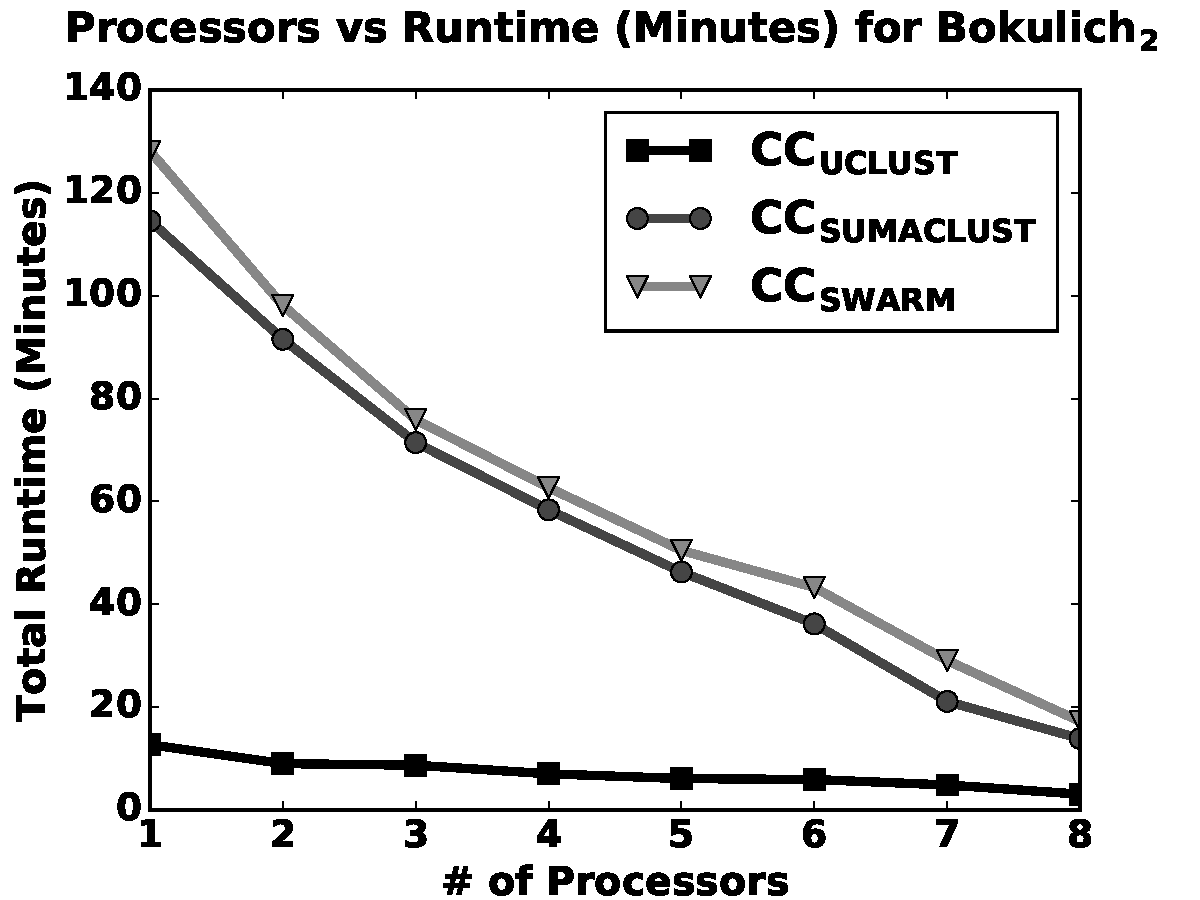
\includegraphics[width=\linewidth]{bokulich_2.pdf}
		\label{fig:bokulich_2}}
	\end{minipage}%
	\hfill%
	\begin{minipage}[t]{0.5\linewidth}
		\subfloat[]{
			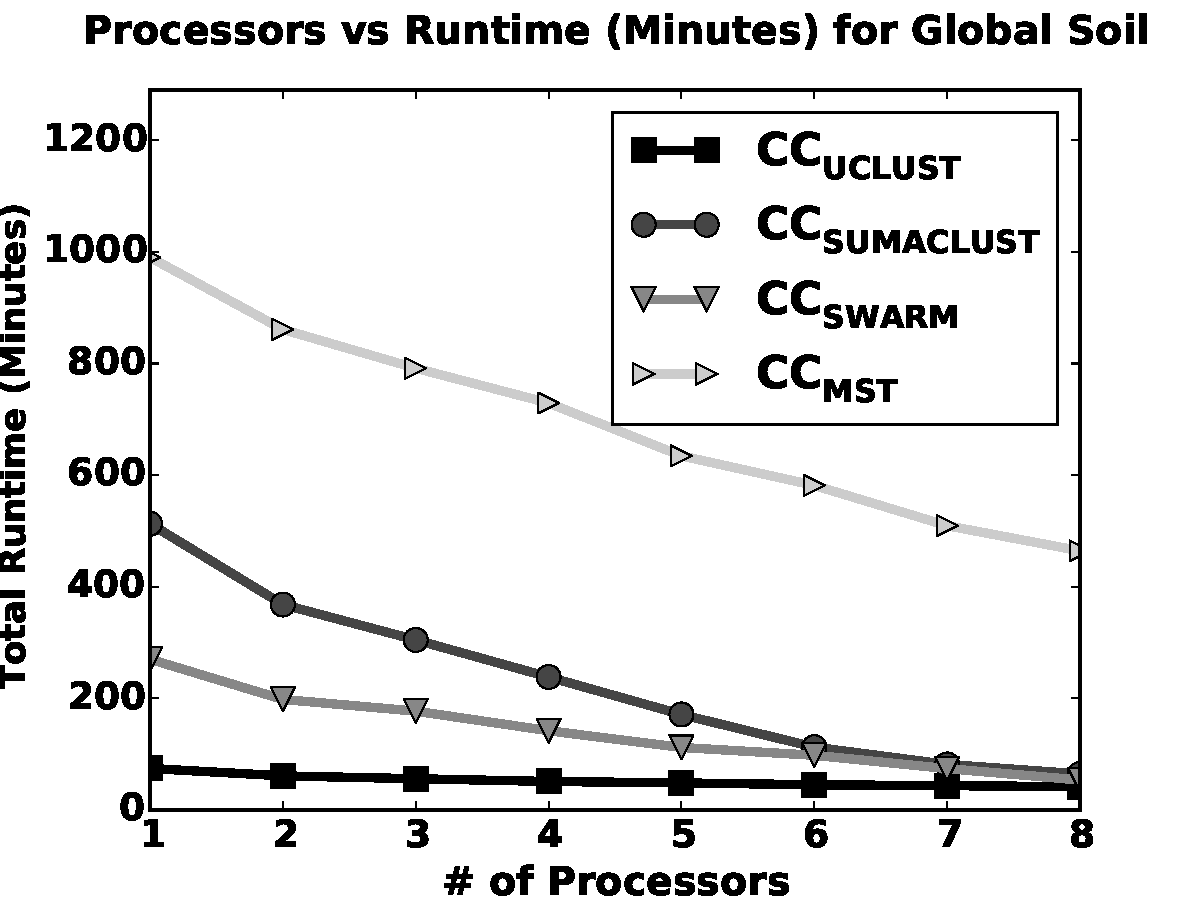
\includegraphics[width=\linewidth]{global_soil.pdf}
			\label{fig:global_soil}}
	\end{minipage}	
	\caption{Effect of number of processors on Runtime of CC$_{UCLUST}$, CC$_{SUMACLUST}$ and CC$_{SWARM}$ for 30M sampled dataset and Global Soil dataset, two of the largest datasets used in this study.}
\end{figure}


\begin{figure}[t]	
	\begin{minipage}[t]{0.5\linewidth}
		\subfloat[]{
			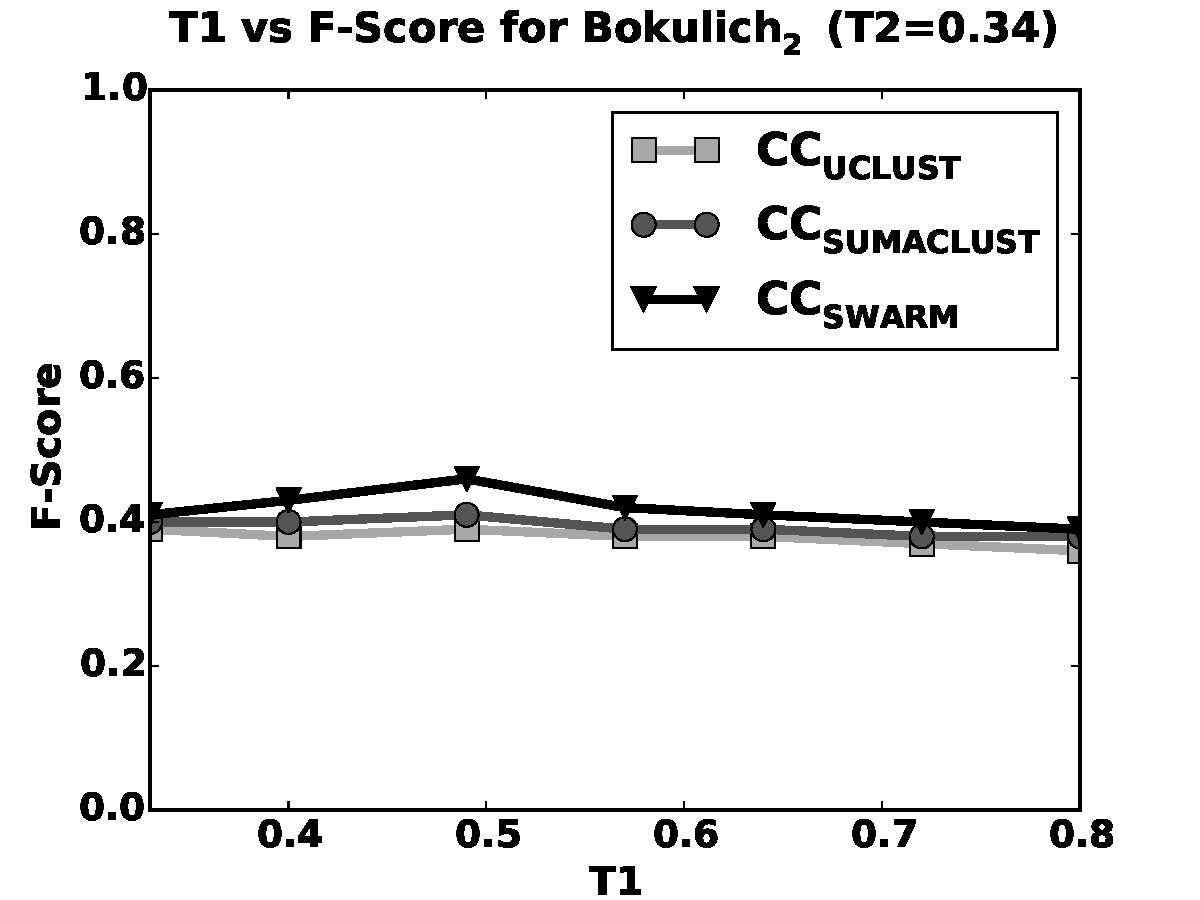
\includegraphics[width=\linewidth]{bokulich_2_T1.pdf}
			\label{fig:bokulich_2_T1}}
	\end{minipage}%
	\hfill%
	\begin{minipage}[t]{0.5\linewidth}
		\subfloat[]{
			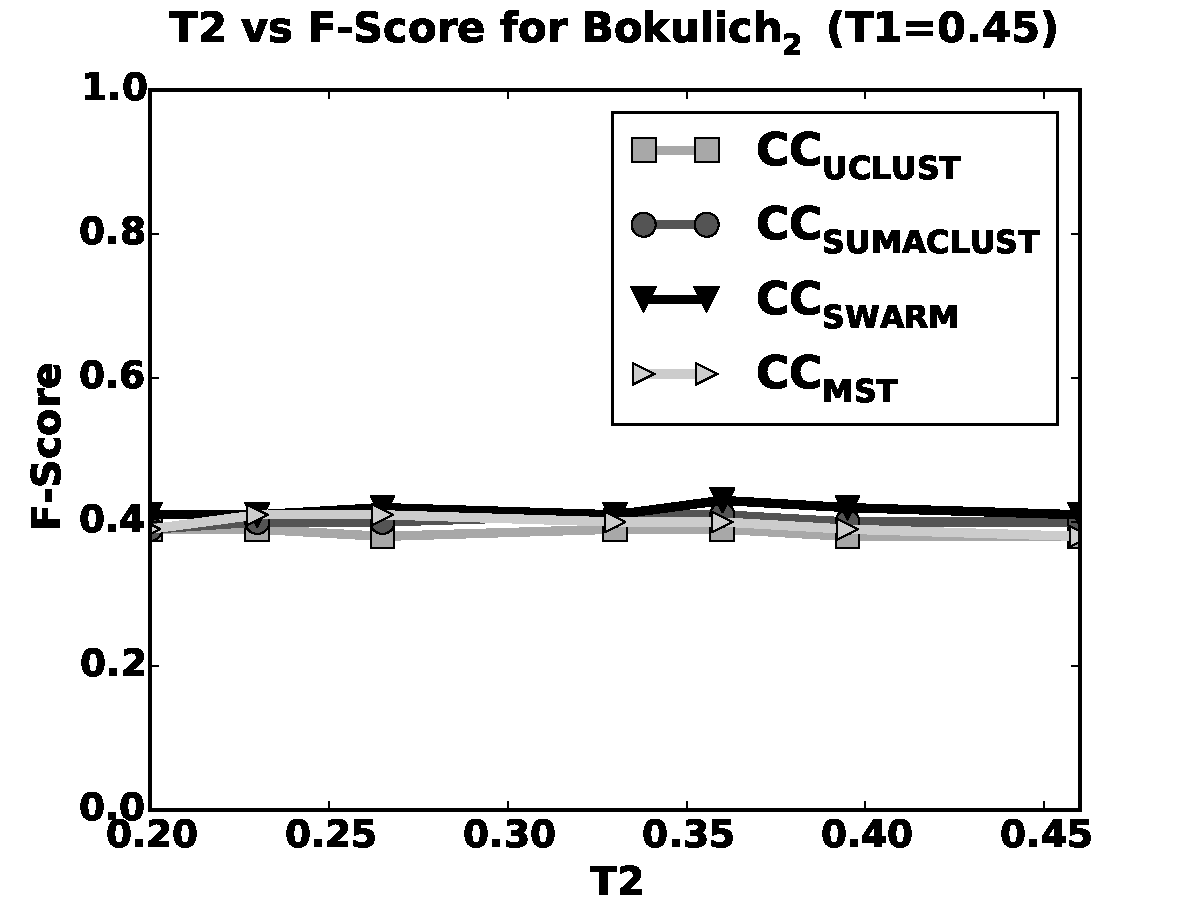
\includegraphics[width=\linewidth]{bokulich_2_T2.pdf}
			\label{fig:bokulich_2_T2}}
	\end{minipage}
	\caption{ \ref{fig:bokulich_2_T1} and \ref{fig:bokulich_2_T2} show effect of varying $T1$ and $T2$ on $F$-scores for the largest synthetic dataset Bokulich$_2$ }	
\end{figure}


\subsection{\textbf{Effect of Varying Number of Processors}}
Figure \ref{fig:bokulich_2}-\ref{fig:global_soil} shows the runtime of CC$_{UCLUST}$, CC$_{SUMACLUST}$ and CC$_{SWARM}$ on two largest benchmarks used in this study - Global Soil and the 30M Liver Cirrhosis dataset. We observe that increasing the number of processors reduces the total runtime. Significant reductions in run time were observed CC$_{SUMACLUST}$ and CC$_{SUMACLUST}$ as 
compared to CC$_{UCLUST}$.   

\subsection{\textbf{Sensitivity Analysis (Varying T1 and T2)}}
Figure \ref{fig:bokulich_2_T1}-\ref{fig:bokulich_2_T2} shows the 
effect of varying $T1$ ($T2$ fixed at 0.34) and $T2$ ($T1$ fixed at 0.45) on F-scores for the Bokulich$_2$ dataset. Reducing $T1$ leads to
comparatively \textit{strict} soft-threshold which will reduce 
repetitions of instances in multiple canopies. For a fixed $T2$ this implies that 
lower $T1$ will yield better canopy assignment. From Figure \ref{fig:bokulich_2_T1} we can say that 
when $T1$'s range is in 0.4 to 0.6 our proposed approach provides better 
F-Scores. On the other hand, increasing $T2$ leads to comparatively \textit{relaxed} tight-threshold for canopies. As a result instances will be prematurely assigned to canopies without waiting for best match. From Figure \ref{fig:bokulich_2_T2} we note that 
when $T2$'  is in between 0.25 to 0.35, 
our proposed approach achieves better F-Scores. Lowering 
$T2$ may lead to higher run time since instances will continue to reappear 
until the $T2$ threshold is satisfied.                   


\section{Conclusion and Future Work}
\label{sec:Conclusion}

We developed a greedy approximate clustering process for any accurate and relatively expensive clustering on large scale metagenome datasets. Our approach takes advantage of the multi-core CPU systems by partitioning the large dataset with a fast and cheap pairwise distance measure and then deploying comparatively expensive clustering in parallel which considers only data points that are inside a partition. Our proposed approach scales well with large datasets and provide significant reduction in computation time. We demonstrate that our approach provides similar outcome in terms of biodiversity metrics, ground truth and taxonomic correlation with corresponding expensive clustering methods.


%\renewcommand{\bibfont}{\footnotesize}
\bibliographystyle{./IEEEtranBST/IEEEtran}
% argument is your BibTeX string definitions and bibliography database(s)
\bibliography{./IEEEtranBST/IEEEabrv,LSH-Canopy-Reference}

% that's all folks
\end{document}


